\documentclass[12pt,a4paper]{article}
\usepackage{amsmath,amsthm,amsfonts,amssymb,amscd}
\usepackage{times}              
% Use Times New Roman
\usepackage{graphicx}           
% Enhanced support for images
\usepackage{float}              
% Improved interface for floating objects
\usepackage{booktabs}           
% Publication quality tables
\usepackage{xcolor}             
% Driver-independent color extensions
\usepackage{geometry}           
% Customize document dimensions
\usepackage{fullpage}           
% all 4 margins to be either 1 inch or 1.5 cm
\usepackage{comment}            
% Commenting
\usepackage{minted}             
% Highlighted source code. Syntax highlighting
\usepackage{listings}           
% Typeset programs (programming code) within LaTeX
\usepackage{lastpage}           
% Reference last page for Page N of M type footers.
\usepackage{fancyhdr}           
% Control of page headers and footers
\usepackage{hyperref}           
% Cross-referencing 
\usepackage[small,bf]{caption}  
% Captions
\usepackage{multicol}
\usepackage{tikz}               
% Creating graphic elements
\usepackage{circuitikz}         
% Creating circuits
\usepackage{verbatim}          
% Print exactly what you type in
\usepackage{cite}               
% Citation
\usepackage[us]{datetime} 
% Various time format
\usepackage{blindtext}
% Generate blind text
\usepackage[utf8]{inputenc}
\usepackage{array}
\usepackage{makecell}
\usepackage{tabularx}
\usepackage{titlesec}

\setlength\parindent{0pt}

%%%%%%%%%%%%%%%%%%%%%%%%%%%%%%%%%%%%%%%%%%%%%%%%%%%%%%%%%%%%%%
\titleformat{\section}
{\color{UM_DarkBlue}\normalfont\large\bfseries}
{\color{UM_DarkBlue}\thesection}{1em}{}

%%%%%%%%%%%%%%%%%%%%%%%%%%%%%%%%%%%%%%%%%%%%%%%%%%%%%%%%%%%%%%
\hypersetup{
    draft=false,
    final=true,
    colorlinks=true,
    citecolor=UM_DarkBlue,
    anchorcolor=yellow,
    linkcolor=UM_DarkBlue,
    urlcolor=UM_DarkBlue,
    filecolor=green,      
    pdfpagemode=FullScreen,
    bookmarksopen=false
    }
    
%%%%%%%%%%%%%%%%%%%%%%%%%%%%%%%%%%%%%%%%%%%%%%%%%%%%%%%%%%%%%%
\lstdefinestyle{Fortran}{
basicstyle=\scriptsize,        % the size of the fonts that are used for the code
  breakatwhitespace=false,         % sets if automatic breaks should only happen at whitespace
  breaklines=false,                 % sets automatic line breaking
  captionpos=b,                    % sets the caption-position to bottom
  commentstyle=\color{mygreen},    % comment style
  extendedchars=true,              % lets you use non-ASCII characters; for 8-bits encodings only, does not work with UTF-8
  keepspaces=true,                 % keeps spaces in text, useful for keeping indentation of code (possibly needs columns=flexible)
  keywordstyle=\color{blue},       % keyword style
  language=[95]Fortran,                 % the language of the code
  numbers=left,                    % where to put the line-numbers; possible values are (none, left, right)
  numbersep=5pt,                   % how far the line-numbers are from the code
  numberstyle=\tiny\color{mygray}, % the style that is used for the line-numbers
  rulecolor=\color{black},         % if not set, the frame-color may be changed on line-breaks within not-black text (e.g. comments (green here))
  showspaces=false,                % show spaces everywhere adding particular underscores; it overrides 'showstringspaces'
  showstringspaces=false,          % underline spaces within strings only
  showtabs=false,                  % show tabs within strings adding particular underscores
  stepnumber=1,                    % the step between two line-numbers. If it's 1, each line will be numbered
  stringstyle=\color{mymauve},     % string literal style
  tabsize=4,                       % sets default tabsize to 2 spaces
  title=\lstname                   % show the filename of files
}

%%%%%%%%%%%%%%%%%%%%%%%%%%%%%%%%%%%%%%%%%%%%%%%%%%%%%%%%%%%%%%%
\definecolor{UM_Brown}{HTML}{3D190D}
\definecolor{UM_DarkBlue}{HTML}{2264B0}
\definecolor{UM_LightBlue}{HTML}{1CA9E1}
\definecolor{UM_Orange}{HTML}{fEB415}




%\newcommand{\tu}[1]{\textup{#1}}
\newcommand{\tu}[1]{\mathrm{#1}}







\newcommand{\ones}{\mathbf 1}
\newcommand{\reals}{{\mbox{\bf R}}}
\newcommand{\integers}{{\mbox{\bf Z}}}
\newcommand{\symm}{{\mbox{\bf S}}}  % symmetric matrices

\newcommand{\nullspace}{{\mathcal N}}
\newcommand{\range}{{\mathcal R}}
\newcommand{\Rank}{\mathop{\bf Rank}}
\newcommand{\Tr}{\mathop{\bf Tr}}
\newcommand{\diag}{\mathop{\bf diag}}
\newcommand{\card}{\mathop{\bf card}}
\newcommand{\rank}{\mathop{\bf rank}}
\newcommand{\conv}{\mathop{\bf conv}}
\newcommand{\prox}{\mathbf{prox}}

\newcommand{\Expect}{\mathop{\bf E{}}}
\newcommand{\Prob}{\mathop{\bf Prob}}
\newcommand{\Co}{{\mathop {\bf Co}}} % convex hull
\newcommand{\dist}{\mathop{\bf dist{}}}
\newcommand{\argmin}{\mathop{\rm argmin}}
\newcommand{\argmax}{\mathop{\rm argmax}}
\newcommand{\epi}{\mathop{\bf epi}} % epigraph
\newcommand{\Vol}{\mathop{\bf vol}}
\newcommand{\dom}{\mathop{\bf dom}} % domain
\newcommand{\intr}{\mathop{\bf int}}
\newcommand{\sign}{\mathop{\bf sign}}

\newcommand{\cf}{{\it cf.}}
\newcommand{\eg}{{\it e.g.}}
\newcommand{\ie}{{\it i.e.}}
\newcommand{\etc}{{\it etc.}}



\usepackage{amsmath}
\begin{document}

\textcolor{UM_Brown}{
    \begin{center}
        \textbf{\Large Near Field Communication}\\
        \vspace{5pt}
        Iot Assignment \\
        \vspace{20pt}
        \textit{P Rahulram} \\
        \vspace{5pt}
        \today
    \end{center}
\vspace{10pt}
\hrule
}



%%%%%%%%%%%%%%% NEW SECTION %%%%%%%%%%%%%%% 
\section*{Introduction}
Near Field Communication (NFC) is a short-range wireless communication technology that enables communication between two devices when they are brought close together. NFC is based on RFID (Radio Frequency Identification) technology and operates at a frequency of 13.56 MHz. It allows for the exchange of data between devices over a distance of less than 10 cm, making it a convenient way to transfer data, make payments, and perform other functions with a simple tap or wave of a device. \\

NFC can be used in IoT devices to enable various applications such as device pairing, mobile payments, access control, and data transfer. It can also be used in wireless charging and inventory management, among others. For example, in IoT-enabled smart homes, an NFC chip can be embedded in a smart lock to allow access to the house with a simple tap of an NFC-enabled smartphone. Similarly, in industrial IoT, NFC tags can be attached to equipment and inventory to track their location and status in real-time.

%%%%%%%%%%%%%%% NEW SECTION %%%%%%%%%%%%%%% 
\section*{Characteristics of NFC}
There are several characteristics that define NFC technology:
\begin{itemize}
    \item \textbf{Short-Range Communication:} NFC operates over a short distance, typically less than 10 cm, which allows for secure and convenient data transfer and other functions between devices.
    \item \textbf{High-Frequency:} NFC operates at a frequency of 13.56 MHz, which is higher than other wireless communication technologies such as Bluetooth and WiFi.
    \item \textbf{Low Power Consumption:} NFC devices use very little power, making it ideal for use in portable and battery-powered devices.
    \item \textbf{Easy to Use:} NFC is simple to use and requires no special knowledge or training. Users can perform various functions, such as making payments or transferring data, with a simple tap or wave of a device.
    \item \textbf{Secure:} NFC uses encryption to protect the data being transferred, and its short-range communication makes it less vulnerable to hacking attempts.
\end{itemize}

%%%%%%%%%%%%%%% NEW SECTION %%%%%%%%%%%%%%% 
\section*{The General Architecture Of NFC Systems}

\begin{figure}[H]
    \centering
    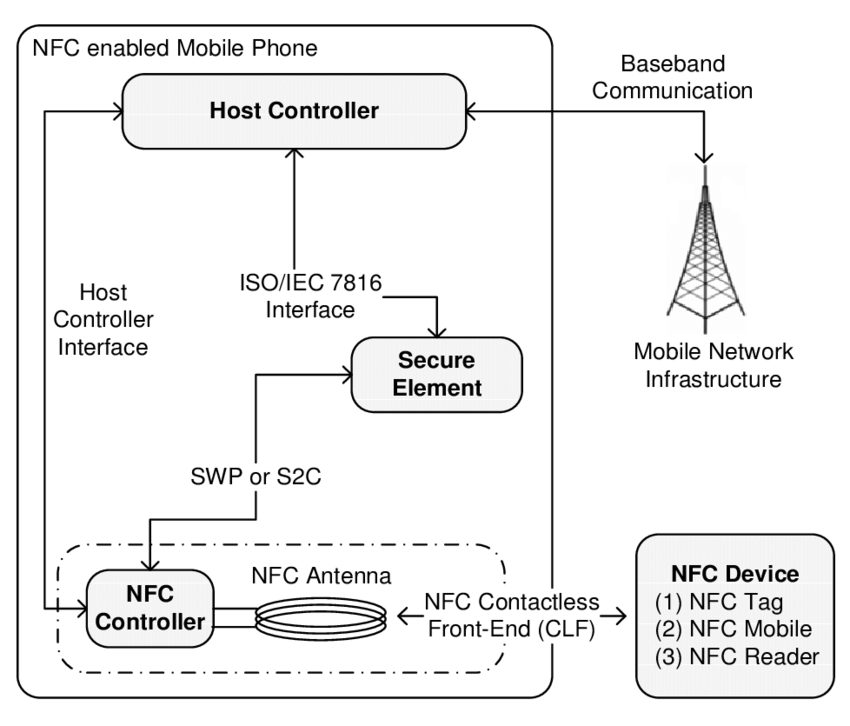
\includegraphics[width=8cm]{nfc.png}
    \caption{General Architecture of NFC enabled Mobile Phones}
\end{figure}

The general architecture of NFC systems typically consists of three main components: the initiator, the target, and the interface device.
\begin{enumerate}
    \item \textbf{Initiator:} The initiator is the device that initiates the communication, such as a smartphone. It typically contains a microcontroller and an NFC transceiver.
    \item \textbf{Target:} The target is the device that responds to the initiator's communication, such as a contactless payment card or an NFC tag. It typically contains an NFC transceiver and a small amount of memory to store data.
    \item \textbf{Interface Device:} The interface device is used to connect the initiator and target devices and facilitates the communication between them. It typically contains an antenna and an NFC controller.
\end{enumerate}

When an initiator and target are brought close together, the interface device detects the proximity of the two devices and establishes a communication link between them. The initiator sends a command to the target, and the target responds with the requested data. The communication link is then terminated when the devices are no longer in proximity. \\

There are several different NFC communication protocols that can be used for the data transfer between initiator and target device. The most widely used protocols are ISO 14443, FeliCa and Mifare, each of them have their own commands and data structure. \\ 

In addition, NFC also has two modes of operation: passive and active. In passive mode, the target device is not powered and relies on the initiator to provide the necessary energy to communicate. In active mode, both the initiator and target devices are powered and can actively initiate and respond to communication. \\ 

Overall, the architecture of NFC systems is designed to be simple, low-power, and secure, making it suitable for a wide range of applications and devices.

%%%%%%%%%%%%%%% NEW SECTION %%%%%%%%%%%%%%% 
\section*{Applications of NFC}
Near Field Communication (NFC) technology can be used in a wide range of applications, including:.
\begin{itemize}
    \item \textbf{Mobile Payments:} NFC can be used for contactless payments, such as making payments with a smartphone or smartwatch at a payment terminal.
    \item \textbf{Healthcare:} NFC can be used in healthcare, such as securely transferring medical information between devices, such as from a patient's smartphone to a doctor's tablet.
    \item \textbf{Transportation and Logistics:} NFC can be used for tracking the location and status of cargo in transportation and logistics.
    \item \textbf{Manufacturing:} NFC can be used for tracking the location and status of equipment and inventory in manufacturing.
    \item \textbf{Smart City:} NFC can be used for various purposes in smart cities such as public transportation, parking, and access control.
\end{itemize}

These are just a few examples of how NFC technology can be used in different areas, the possibilities are endless and more use cases are expected to appear as the technology evolves.

%%%%%%%%%%%%%%% NEW SECTION %%%%%%%%%%%%%%% 
\section*{Drawbacks and Security Risks of NFC}
While NFC technology offers many benefits and conveniences, there are also some drawbacks and security risks to consider.
\begin{itemize}
    \item \textbf{Limited Range:} The range of NFC communication is limited, typically less than 10cm, which can be a drawback for certain applications, such as inventory management or tracking, where a longer range is needed.
    \item \textbf{Interference:} NFC communication can be affected by interference from other devices that operate in the same frequency range, such as other NFC devices or wireless routers.
    \item \textbf{Security Risks:} NFC transactions can be vulnerable to "skimming" attacks, where a malicious device is used to intercept data from an NFC transaction, such as credit card information. To avoid this, it's important to use secure and encrypted protocols for NFC transactions and to be aware of the security features of your NFC-enabled device.
    \item \textbf{Privacy Risks:} NFC tags can be used to track an individual's location and behavior, which can be a privacy concern. To avoid this, it's important to be aware of the type of data that is stored on NFC tags, and to disable NFC on your device when it is not in use.
    \item \textbf{Device Compatibility:} Not all devices are NFC-enabled, which can limit the functionality and convenience of NFC.
\end{itemize}

Overall, while NFC technology offers many benefits, it's important to be aware of its potential drawbacks and security risks and take the necessary precautions to protect your devices and personal information.

\end{document}
